\documentclass[16pt, letterpaper]{article}
\usepackage{amsmath}
\usepackage{algorithm}
\usepackage{tikz}
\usetikzlibrary{calc}
\newcounter{nodeidx}
\setcounter{nodeidx}{1}
\newcommand{\nodes}[1]{%
    \foreach \num in {#1}{
      \node[minimum size=6mm, draw, rectangle] (\arabic{nodeidx}) at (\arabic{nodeidx},0) {\num};
      \stepcounter{nodeidx}
    }
    % reset counter to re-use command
    \setcounter{nodeidx}{1}
}
\newcommand{\brckt}[4]{% from, to, lvl, text
  \draw (#1.south west) ++($(-.1, -.1) + (-.1*#3, 0)$) -- ++($(0,-.1) + (0,-#3*1.25em)$) -- node [below] {#4} ($(#2.south east) + (.1,-.1) + (.1*#3, 0) + (0,-.1) + (0,-#3*1.25em)$) -- ++($(0,#3*1.25em) + (0,.1)$);%
}


\usepackage[noend]{algpseudocode}
\usepackage{comment}
\title{Gina Cody Shool of Computer Science and Software Engineering \\Concordia University
\\COMP 352: Data Structure and Algorithms }
\author{Student: Duc Nguyen}
\date{}

\begin{document}

\begin{titlepage}
\maketitle
\end{titlepage}
\tableofcontents

\section{Double-stack array} 
\textbf{NOTE: All the Java implementation of this question is in the folder Implementation. This is out of scope for this assignment, but it will help anyone reading this get a better understanding.}
\subsection{Case 1: }
Fairness in space allocation to the two stacks is required. In that sense, if Stack1 for instance use all its allocated space, while Stack 2 still has some space; insertion into Stack 1 cannot be made, even though there are still some empty elements in the array.

\subsubsection*{A. Description}
In this scenario, the array could be implemented by allocating the range from starting index to the maximum capacity index to be the reserved space for Stack 1 (left-to-right order). 
While stack 2 takes place from the last index of the array, goes left until it reaches its maximum capacity (right-to-left order).

\begin{tikzpicture}
    \pgftransparencygroup
    \nodes{0,1,$\dots$,i, $\dots$, $\dots$, j, $\dots$, 1, 0}
    \endpgftransparencygroup
%----End Line 1
    \pgftransparencygroup
    \brckt{1}{4}{0}{Fixed-capacity Stack 1}
    \endpgftransparencygroup
    
    \pgftransparencygroup
    \brckt{7}{10}{0}{Fixed-capacity Stack 2}
    \endpgftransparencygroup
%----End Line 2 
    \pgftransparencygroup
    \brckt{1}{10}{1}{Array}
    \endpgftransparencygroup
\end{tikzpicture}

\textit{Illustration of the implementation in this case. The index is of stack that it belongs to, not the "real" index of the array. }

\textbf{Global variables:}
\begin{itemize} 
    \item array: the array itself
    \item arrayLength: The length of the array
    \item headStack1(i): The index of the last element in Stack 1. (starts from -1 when the stack is empty)
    \item stack1Capacity: the fixed given capacity of Stack 1.
    \item headStack2(j): The index of the last element in Stack 2. (starts from arrayLength when the stack is empty)
    \item stack2Capacity: the fixed given capacity of Stack 2.
\end{itemize}

\subsubsection*{B. Algorithms for push(), pop(), size(), isEmpty(), is Full()}
%  PUSH METHODS
\begin{algorithm} [H]
\caption{Push Element to Stack 1}
\begin{algorithmic}[1]
	\Procedure{PushStack1(element)} {}
	\If{$isStack1Full() = false$}
		\State$headStack1 \gets \textit{headStack1} + 1$
		\State$array[headStack1] \gets \textit{element}$
	\Else
		\State\textit{throw FullStackException}
	\EndIf
	\EndProcedure
\end{algorithmic}
\end{algorithm}

\begin{algorithm} [H]
\caption{Push Element to Stack 2}
\begin{algorithmic}[1]
    \Procedure{PushStack2(Element)} {}
    \If{$isStack2Full() = false$}
        \State $headStack2 \gets \textit{headStack2} - 1$
        \State $array[headStack2] \gets \textit{element}$
    \Else 
        \State\textit{throw FullStackException}
    \EndIf
    \EndProcedure
\end{algorithmic}
\end{algorithm}
% ---------------------

% POP METHODS
\begin{algorithm} [H]
\caption{Pop Element out of Stack 1. Return the popped element}
\begin{algorithmic}[1]
    \Procedure{popStack1()}{}
    \If {$isStack1Empty() = false$}
        \State $temp \gets \textit{array[headStack1]}$
        \State $array[headStack1] \gets \textit{null}$
        \State $headStack1 \gets \textit{headStack1 - 1}$ 
        \State \Return $temp$
    \Else
        \State \textit{throw EmptyStackException}
    \EndIf
    \EndProcedure
\end{algorithmic}
\end{algorithm}

\begin{algorithm} [H]
\caption{Pop Element out of Stack 2. Return the popped element}
\begin{algorithmic}[1]
    \Procedure{popStack2()}{}
    \If {$isStack2Empty() = false$}
        \State $temp \gets \textit{array[headStack2]}$
        \State $array[headStack2] \gets \textit{null}$
        \State $headStack2 \gets \textit{headStack2 + 1}$
        \State \Return $temp$
    \Else
        \State \textit{throw EmptyStackException}
    \EndIf
    \EndProcedure
\end{algorithmic}
\end{algorithm}
%------------------

% SIZE
\begin{algorithm} [H]
\caption{Return an integer indicates the current size of Stack 1}
\begin{algorithmic}
    \Procedure{sizeStack1()}{}
    \State \Return $\textit{headStack1 + 1}$
    \EndProcedure
\end{algorithmic}
\end{algorithm}

\begin{algorithm} [H]
\caption{Return an integer indicates the current size of Stack 2}
\begin{algorithmic}
    \Procedure{sizeStack2()}{}
    \State \Return $\textit{arrayLength - headStack2}$
    \EndProcedure
\end{algorithmic}
\end{algorithm}
%------------------

% isEmpty methods
\begin{algorithm} [H]
\caption{Return a boolean value indicates whether or not Stack 1 is empty}
\begin{algorithmic}
    \Procedure{isStack1Empty()}{}
    \If{$headStack1 = -1$}
    \State \Return $\textit{true}$
    \Else
    \State \Return $\textit{false}$
    \EndIf
    \EndProcedure
\end{algorithmic}
\end{algorithm}

\begin{algorithm} [H]
\caption{Return a boolean value indicates whether or not Stack 2 is empty}
\begin{algorithmic}
    \Procedure{isStack2Empty()}{}
    \If{$headStack2 = arrayLength$}
    \State \Return $\textit{true}$
    \Else
    \State \Return $\textit{false}$
    \EndIf
    \EndProcedure
\end{algorithmic}
\end{algorithm}
%-----------------

% isFull methods
\begin{algorithm} [H]
\caption{Return a boolean value indicates whether or not Stack 1 is full}
\begin{algorithmic}
    \Procedure{isStack1Full()}{}
    \If{$sizeStack1() = stack1Capacity$} 
    \State \Return $\textit{true}$
    \Else
    \State \Return $\textit{false}$
    \EndIf
    \EndProcedure
\end{algorithmic}
\end{algorithm}

\begin{algorithm} [H]
\caption{Return a boolean value indicates whether or not Stack 2 is full}
\begin{algorithmic}
    \Procedure{isStack2Full()}{}
    \If{$sizeStack2() = stack2Capacity$} 
    \State \Return $\textit{true}$
    \Else
    \State \Return $\textit{false}$
    \EndIf
    \EndProcedure
\end{algorithmic}
\end{algorithm}
%-------------

\subsubsection*{C. Big-O complexity}
Since every algorithm performs with a constant time: 
\begin{itemize}
    \item Push() - $O(1)$
    \item Pop() - $O(1)$
    \item Size() - $O(1)$
    \item isEmpty() - $O(1)$
    \item isFull() - $O(1)$
\end{itemize}

\subsubsection*{D. Big-$\Omega()$ complexity}
\begin{itemize}
    \item Push() - $\Omega(1)$
    \item Pop() - $\Omega(1)$
    \item Size() - $\Omega(1)$
    \item isEmpty() - $\Omega(1)$
    \item isFull() - $\Omega(1)$
\end{itemize}

%------------------PROBLEM 1: CASE 2
\subsection{Case 2: }
Space is critical; so you should use all available elements in the array if needed. In other words, the two stacks may not finally get the same exact amount of allocation, as one of them may consume more elements (if many push() operations are performed for instance into that stack first).

\subsubsection*{A. Description}
The ADT can be implemented by the same way as the previous case. However, in this case, it keeps pushing new element into both stacks without a fixed limit for the capacity. A stack is only full when the array is full of elements.

\begin{tikzpicture}
    \pgftransparencygroup
    \nodes{0,1,$\dots$,i, j, $\dots$, $\dots$, $\dots$, 1, 0}
    \endpgftransparencygroup
%----End Line 1
    \pgftransparencygroup
    \brckt{1}{4}{0}{Dynamic-capacity Stack 1}
    \endpgftransparencygroup
    
    \pgftransparencygroup
    \brckt{5}{10}{0}{Dynamic-capacity Stack 2}
    \endpgftransparencygroup
%----End Line 2 
    \pgftransparencygroup
    \brckt{1}{10}{1}{Array}
    \endpgftransparencygroup
\end{tikzpicture}
\\
\textit{Illustration of the implementation in this case. The index is of stack that it belongs to, not the "real" index of the array.}

\textbf{Global variables:}
\begin{itemize} 
    \item array: the array itself
    \item arrayLength: The length of the array
    \item headStack1: The index of the last element in Stack 1. (starts from -1 when the stack is empty)
    \item headStack2: The index of the last element in Stack 2. (starts from arrayLength when the stack is empty)
\end{itemize}

\subsubsection*{B. Algorithms for push(), pop(), size(), isEmpty(), is Full()}
%  PUSH METHODS
\begin{algorithm} [H]
\caption{Push Element to Stack 1}
\begin{algorithmic}[1]
	\Procedure{PushStack1(element)} {}
	\If{$isFull()= false$}
		\State$headStack1 \gets \textit{headStack1} + 1$
		\State$array[headStack1] \gets \textit{element}$
	\Else
		\State\textit{throw FullStackException}
	\EndIf
	\EndProcedure
\end{algorithmic}
\end{algorithm}

\begin{algorithm} [H]
\caption{Push Element to Stack 2}
\begin{algorithmic}[1]
    \Procedure{PushStack2(Element)} {}
    \If{$isFull() = false$}
        \State $headStack2 \gets \textit{headStack2} - 1$
        \State $array[headStack2] \gets \textit{element}$
    \Else 
        \State\textit{throw FullStackException}
    \EndIf
    \EndProcedure
\end{algorithmic}
\end{algorithm}
% ---------------------

% POP METHODS
\begin{algorithm} [H]
\caption{Pop Element out of Stack 1. Return the popped element}
\begin{algorithmic}[1]
    \Procedure{popStack1()}{}
    \If {$isStack1Empty() = false$}
        \State $temp \gets \textit{array[headStack1]}$
        \State $array[headStack1] \gets \textit{null}$
        \State $headStack1 \gets \textit{headStack1 - 1}$ 
        \State \Return $temp$
    \Else
        \State \textit{throw EmptyStackException}
    \EndIf
    \EndProcedure
\end{algorithmic}
\end{algorithm}

\begin{algorithm} [H]
\caption{Pop Element out of Stack 2. Return the popped element}
\begin{algorithmic}[1]
    \Procedure{popStack2()}{}
    \If {$isStack2Empty() = false$}
        \State $temp \gets \textit{array[headStack2]}$
        \State $array[headStack2] \gets \textit{null}$
        \State $headStack2 \gets \textit{headStack2 + 1}$
        \State \Return $temp$
    \Else
        \State \textit{throw EmptyStackException}
    \EndIf
    \EndProcedure
\end{algorithmic}
\end{algorithm}
%------------------

% SIZE
\begin{algorithm} [H]
\caption{Return an integer indicates the size of Stack 1}
\begin{algorithmic}
    \Procedure{sizeStack1()}{}
    \State \Return $\textit{headStack1 + 1}$
    \EndProcedure
\end{algorithmic}
\end{algorithm}

\begin{algorithm} [H]
\caption{Return an integer indicates the size of Stack 2}
\begin{algorithmic}
    \Procedure{sizeStack2()}{}
    \State \Return $\textit{arrayLength - headStack2}$
    \EndProcedure
\end{algorithmic}
\end{algorithm}
%------------------

% isEmpty methods
\begin{algorithm} [H]
\caption{Return a boolean value indicates whether or not Stack 1 is empty}
\begin{algorithmic}
    \Procedure{isStack1Empty()}{}
    \If{$headStack1 = -1$}
    \State \Return $\textit{true}$
    \Else
    \State \Return $\textit{false}$
    \EndIf
    \EndProcedure
\end{algorithmic}
\end{algorithm}

\begin{algorithm} [H]
\caption{Return a boolean value indicates whether or not Stack 2 is empty}
\begin{algorithmic}
    \Procedure{isStack2Empty()}{}
    \If{$headStack2 = arrayLength$}
    \State \Return $\textit{true}$
    \Else
    \State \Return $\textit{false}$
    \EndIf
    \EndProcedure
\end{algorithmic}
\end{algorithm}
%-----------------

% isFull method
\textbf{When the size of both stack is dynamic, the only time a stack is full is when the array is full.}
\begin{algorithm} [H]
\caption{Return a boolean value indicates whether or not a stack is full}
\begin{algorithmic}
    \Procedure{isFull()}{}
    \If{$headStack1 + 1 = headStack2$} 
    \State \Return \textit{true}
    \Else
    \State \Return \textit{false}
    \EndIf
    \EndProcedure
\end{algorithmic}
\end{algorithm}
%-----------------

\subsubsection*{C. Big-O complexity}
Since there was no loop, or recursive calls in every implemented method, and every algorithm performs in a constant amount of time:
\begin{itemize}
    \item Push() - $O(1)$
    \item Pop() - $O(1)$
    \item Size() - $O(1)$
    \item isEmpty() - $O(1)$
    \item isFull() - $O(1)$
\end{itemize}

\subsubsection*{D. Big-$\Omega$complexity}
\begin{itemize}
    \item Push() - $\Omega(1)$
    \item Pop() - $\Omega(1)$
    \item Size() - $\Omega(1)$
    \item isEmpty() - $\Omega(1)$
    \item isFull() - $\Omega(1)$
\end{itemize}

\subsection{Concerning the possibility of a 3-stack array}
\begin{itemize}
    \item \textbf{Case 1:}
    It is possible to implement a three-stack array. The third stack will lie between the first stack, and the second stack. In this case, the complexity will not change significantly since every stack has reserved its own space inside the array.
    
\begin{tikzpicture}
    \pgftransparencygroup
    \nodes{0, $\dots$,i, 0, $\dots$, h ,$\dots$, $\dots$, k, $\dots$, 0}
    \endpgftransparencygroup
%----End Line 1
    \pgftransparencygroup
    \brckt{1}{3}{0}{Fixed-size Stack 1}
    \endpgftransparencygroup
    
    \pgftransparencygroup
    \brckt{4}{6}{0}{new Stack 3}
    \endpgftransparencygroup
    
    \pgftransparencygroup
    \brckt{9}{11}{0}{Fixed-size Stack 2}
    \endpgftransparencygroup
%----End Line 2 
    \pgftransparencygroup
    \brckt{1}{11}{1}{Array}
    \endpgftransparencygroup
\end{tikzpicture}

\textit{Illustration of one possible implementation in this case. The index is of stack that it belongs to, not the "real" index of the array.}

    \item \textbf{Case 2:}
    It is possible to implement a three-stack array. To optimize all space inside the array, the new third stack starts right after the end of the first stack (after headStack1) , but it must end before the end of stack 2 (before headStack2). This leads to a significant change in time complexity since the stack 3 will have to shift all its elements every time there is a new push or pop operation in stack 1. 
    
\begin{tikzpicture}
    \pgftransparencygroup
    \nodes{0, 1, $\dots$,i, 0, $\dots$, h, k, $\dots$, 1, 0}
    \endpgftransparencygroup
%----End Line 1
    \pgftransparencygroup
    \brckt{1}{4}{0}{Dynamic-size Stack 1}
    \endpgftransparencygroup
    
    \pgftransparencygroup
    \brckt{5}{7}{0}{new Stack 3}
    \endpgftransparencygroup
    
    \pgftransparencygroup
    \brckt{8}{11}{0}{Dynamic-size Stack 2}
    \endpgftransparencygroup
%----End Line 2 
    \pgftransparencygroup
    \brckt{1}{11}{1}{Array}
    \endpgftransparencygroup
\end{tikzpicture}

\textit{Illustration of one possible implementation in this case. The index is of stack that it belongs to, not the "real" index of the array.}
\end{itemize}

\section{Antique dealer}
\subsection{Pseudo code of max() function in a stack based array}
\textbf{Variables:}
\begin{itemize}
    \item \textit{stack:} the stack itself implemented in the array
    \item \textit{headStack:} the last index of the stack inside the array.
\end{itemize}
\begin{algorithm} [H]
\caption{Return the maximum value of the inventory}
\begin{algorithmic}[1]
    \Procedure{max()}{}
    \State $max \gets stack[0]$
    \For{$k \gets 1$ to $headStack$}
    \If{$stack[k] > max$}
    \State $max \gets stack[k]$
    \EndIf
    \EndFor
    \State \Return max
    \EndProcedure
\end{algorithmic}
\end{algorithm}

\subsection{Big-O complexity}
Since the algorithm has to loop through every existing element inside the stack, the complexity of the algorithm is O(n).

\subsection{Possible to have \underline{all}  3 methods (push(), pop(), and max()) be designed to have O(1)?}
It is possible to have all 3 methods push(), pop() and max() to have O(1). It could be implemented by using a singly linked list. Each \textit{node} inside the linked list would contain a variable \emph{Max} to keep track of the max value each time a new element is pushed in, along with \emph{Next} serves as a poiner, links to the next node. 
In addition, the top of the stack is being implemented at the \textit{Head} of the linked list.
\\
\textbf{Demonstration}
\begin{algorithm} [H]
\caption{Push new element into the inventory}
\begin{algorithmic}[1]
    \Procedure{push(newValue)}{}
    \State $temp \gets Node(newValue)$ \Comment{Create a new Node with newValue}
    \If{$head \neq null$} 
    \State $temp.max \gets maxOf(head.max, newValue)$
    \State $temp.next \gets head$
    \State $head \gets temp$
    \Else\Comment{Stack is currently empty}
    \State $temp.max \gets newValue$ 
    \State $head \gets temp$
    \EndIf
    \EndProcedure
\end{algorithmic}
\end{algorithm}

\begin{algorithm} [H]
\caption{Pop and return the last element}
\begin{algorithmic}[1]
    \Procedure{pop()}{}
    \If {$head = null$}\Comment{The stack is currently empty}
    \State \Return null
    \Else 
    \State $temp \gets \textit{head}$
    \State $head \gets \textit{head.next}$
    \State \Return temp
    \EndIf
    \EndProcedure
\end{algorithmic}
\end{algorithm}

\begin{algorithm}[H]
\caption{Return the max value in the inventory}
\begin{algorithmic}[1]
\Procedure{max()}{}
    \If{$head = null$} \Return 0 \Comment{The stack currently is empty} 
    \Else 
    \State \Return \textit{head.max}
    \EndIf
\EndProcedure
\end{algorithmic}
\end{algorithm}

\textbf{Note:} All the algorithms here were implemented in the folder \textit{Implementation} to give readers better understanding.

\section{Evaluate complexity's relationship}
\begin{tabular}{l l l}
a. & $f(n) = {\log^3 n}$ & $g(n) = \sqrt n$ \\
b. & $f(n) = n\sqrt n + \log n$ & $g(n) = \log n^2 $ \\
c. & $f(n) = n $ & $g(n) = \log^2 n$ \\
d. & $f(n) = \sqrt n $ & $g(n) = 2^(\sqrt {\log n})$ \\
e. & $f(n) = 2^n $ & $g(n) = 3^n$
\end{tabular}

\textbf{a}. $f(n) = {\log^3 n}$ is of power 3 while $\sqrt n$ is a function of square root. Thus, the growth rate of f(n) is slower than g(n). \textbf{$\longrightarrow f(n)$ is of $O(g(n))$}

\textbf{b}. $f(n) = n\sqrt n + \log n$  has a greater growth rate when comparing with growth rate of $g(n) = \log n^2 $. \textbf{$\longrightarrow f(n)$ is of $\Omega(g(n))$}

\textbf{c}. $f(n) = n $ is a function with linear growth rate while $g(n) = \log^2 n$ is a function of log. The linear growth is faster than log function. Thus, \textbf{$f(n)$ is of $\Omega(g(n))$} 

\textbf{d}. While $f(n) = \sqrt n$ is of square root function, the function $g(n) = 2^(\sqrt{\log n})$ is of exponential. However, the exponential of g(n) is a square root function. That leads to a slightly slower rate of growth in g(n). \textbf{$\longrightarrow f(n)$ is of $\Omega(g(n))$}

\textbf{e}. $f(n) = 2^n$ is an exponential function with base 2; while $g(n) = 3^n$ is an exponential function with base 3. Thus, $g(n) > f(n) \forall n \geq 1$. \textbf{$\longrightarrow f(n)$ is of O(g(n)) }

\section{Remove duplicate elements}
\subsection{Description}
Create a stack firstly. Then make a loop through each element inside the given array. If the element was already pushed into the array, then the program will not re-push it again. In other word, the program only pushes the element which is not the duplication of any existing elements inside the Stack. After finish pushing elements into the Stack, create a new array which has the same size with the Stack. Then, the algorithm pops each element in the Stack into the array in reverse order (to guarantee the order in the new array is the same as the given one).

\begin{tikzpicture}
    \pgftransparencygroup
    \nodes{22, 61, -10 , 61, 10, 12, 9, 61, 9, 77, 5}
    \endpgftransparencygroup
%----End Line 1
% GIVEN ARRAY
    \pgftransparencygroup
    \brckt{1}{11}{1}{Given Array}
    \endpgftransparencygroup
\end{tikzpicture}
\\
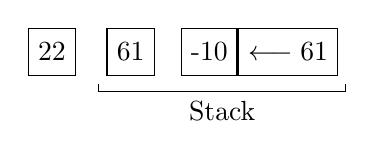
\begin{tikzpicture}
%----Stack 
    \pgftransparencygroup
    \nodes{22, 61, -10, $\longleftarrow 61$}
    \endpgftransparencygroup
    \pgftransparencygroup
    \brckt{1}{3}{0}{Stack}
    \endpgftransparencygroup
\end{tikzpicture}
\Comment{61 was already in the stack $\longrightarrow$ No push}
\\
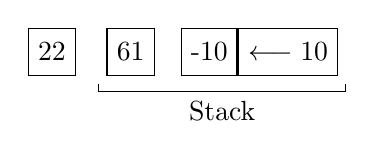
\begin{tikzpicture}
%----Stack 
    \pgftransparencygroup
    \nodes{22, 61, -10, $\longleftarrow 10$}
    \endpgftransparencygroup
    \pgftransparencygroup
    \brckt{1}{3}{0}{Stack}
    \endpgftransparencygroup
\end{tikzpicture}
\Comment{10 was not in the stack $\longrightarrow$ Push(10)}
\\
\textbf{Continue the process until the end of the given array $\dots$}
\\
\begin{tikzpicture}
%----Stack 
    \pgftransparencygroup
    \nodes{22, 61, -10, 10, 12, 9, 77, 5}
    \endpgftransparencygroup
    \pgftransparencygroup
    \brckt{1}{8}{0}{Stack after pushing}
    \endpgftransparencygroup
\end{tikzpicture}
\\
\textbf{Popping each element into the new array in reverse order}
\\
\begin{tikzpicture}
%----Stack 
    \pgftransparencygroup
    \nodes{22, 61, -10, 10, 12, 9, 77, 5$\longrightarrow$}
    \endpgftransparencygroup
    \pgftransparencygroup
    \brckt{1}{8}{0}{Stack being popped}
    \endpgftransparencygroup
\end{tikzpicture}

\algnewcommand\algorithmicforeach{\textbf{for each}}
\algdef{S}[FOR]{ForEach}[1]{\algorithmicforeach\ #1\ \algorithmicdo}

\begin{algorithm}[H]
\caption{Receive input as an integer \textit{array}, and return output as a new array which has no duplicate items.}
\begin{algorithmic}[1]
\Procedure{removeDuplicate(int[] array)}{}
\State $stack \gets \textit{new Stack of Integer}$
\ForEach {$element \in \mathcal  Array$}\Comment{Pushing elements into the Stack}
\If{$stack.contain(element) == false$}
\State \textit{stack.push(element)}
\EndIf
\EndFor

\State $result \gets \text{new int[stack.size()]}$\Comment{Popping Stack elements to \textit{result}}
\For{$(i \gets result.length - 1; i \geq 0; i--)$}
\State $result[i] = stack.pop()$
\EndFor
\State \Return $result$

\EndProcedure
\end{algorithmic}
\end{algorithm}

\subsection{Big-O Complexity}
Big-O complexity of this solution would be $O(n^2)$ since the algorithm has to loop through each element inside the array once \textbf{(n)}. Each element has to be compared to each existing element inside the stack \textbf{(n)} in order to make decision whether or not push this new element into the stack. Lastly, popping every element inside the stack to the new result array is of \textbf{O(n)}. Thus, it is $O(n*n + n) = O(n^2)$.

\subsection{Big-$\Omega$ Complexity}
Best case scenario in this situation is when the algorithm tries to determine should the element be pushed to Stack or not, the duplicate item is already at the front of the Stack; thus, there is no need to check other elements. Therefore, best case scenario is when the given array is full of duplicate items. As a result, the time complexity of the algorithm is of $\Omega(n)$.

\subsection{Big-O \emph{space} complexity}
The worst case scenario for the memory is when there is no duplication in the given array. Then the size of the Stack is the same with the array. As a result, the algorithm space complexity is of \textbf{O(n)}

\end{document}
